\subsection*{Retrospective ablation and error-mechanism checks}
The previous comparison changed both training scenes and clip-checkpoint selection. A completed $2\times2$ analysis now crosses original/controlled training data with F1/balanced-accuracy clip selection, separately for mean and attention pooling. Twelve new runs fill the missing cells; twelve retained runs provide the existing cells. All use seeds 5305--5307, the same encoder and optimiser, timestamp bins, and validation-balanced frame calibration. No test score changes the original architecture winner. This is retrospective development analysis on the same inspected test tracks.
\begin{table}[H]\centering\small
\caption{Retrospective factorial comparison on the controlled test distribution. Means and sample SD over three seeds. All cells use the same validation-balanced frame threshold protocol. The original architecture winner is unchanged.}\label{tab:factorial}
\begin{tabular}{lllrr}\toprule
Model & Training data & Clip selection & Frame BA & Micro F1 \\\midrule
baseline & original & F1 & $0.559 \pm 0.013$ & 0.636 \\
baseline & original & BA & $0.568 \pm 0.006$ & 0.676 \\
baseline & controlled & F1 & $0.589 \pm 0.005$ & 0.655 \\
baseline & controlled & BA & $0.589 \pm 0.005$ & 0.655 \\
attention & original & F1 & $0.570 \pm 0.013$ & 0.643 \\
attention & original & BA & $0.584 \pm 0.007$ & 0.681 \\
attention & controlled & F1 & $0.620 \pm 0.003$ & 0.697 \\
attention & controlled & BA & $0.629 \pm 0.011$ & 0.702 \\
\bottomrule\end{tabular}\end{table}
Under fixed balanced selection, attention's controlled-test frame BA rises from \OriginalAttentionBA{} with original training scenes to \ControlledAttentionBABA{} with controlled training. Under F1 selection, controlled training reaches \ControlledAttentionFoneBA{}. Thus the gain is not explained solely by changing clip selection. The data factor also changes scene count and optimiser exposure: this is evidence for the complete training-data condition, not a pure causal estimate of acoustic augmentation. Paired seed contrasts are in \code{results/ablation_v4/summary.json}.

Attention exceeds mean on all four test tracks. The unweighted controlled-track BA difference is \TrackDelta{}; leaving out any one track gives \TrackLooLow{}--\TrackLooHigh{}. These are descriptive robustness values, not confidence limits or proof of population generalisation.

Among bins with bass absent, mean bass FPR across attention seeds is \BassFprDrumsOn{} when drums are active (1235 reference bins), versus \BassFprDrumsOff{} when drums are absent (1055 bins). Reference bins are correlated and are not independent recordings. Repeating predictions over seeds does not multiply these denominators. Contextual confusion, arrangement, masking and the intervention construction are possible explanations; this association does not prove which acoustic evidence the model causally uses.
\begin{figure}[H]\centering
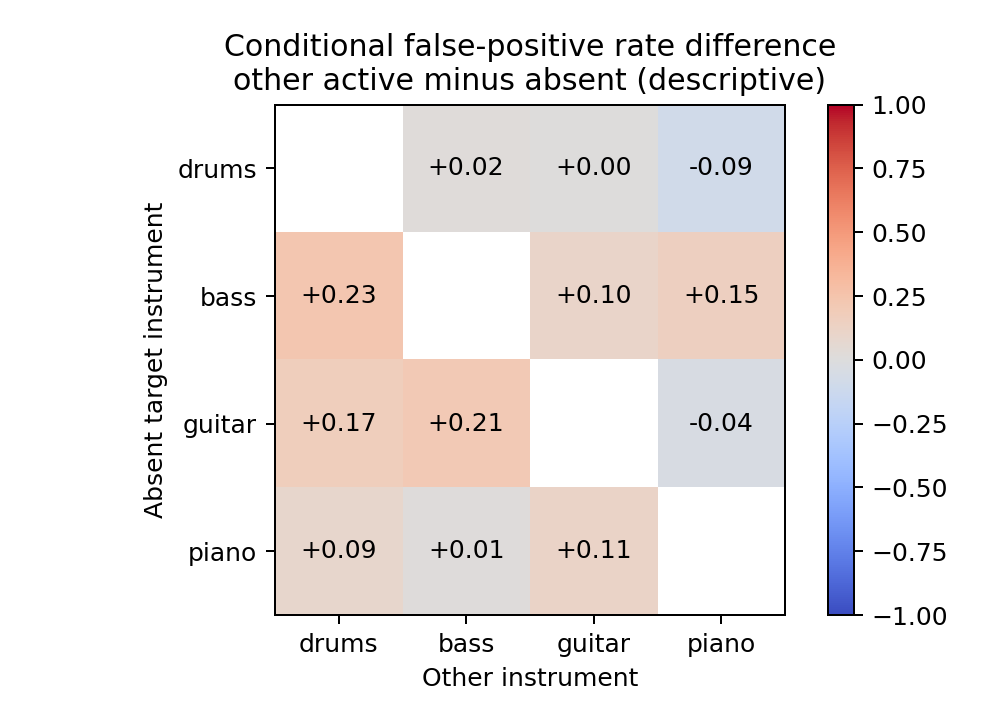
\includegraphics[width=.65\linewidth]{figures/conditional_fpr_v4.png}
\caption{Conditional FPR difference: the target family is absent, while the column family is active versus absent. Mean over three attention seeds; both conditions require at least 20 bins. The diagonal is undefined. These exploratory comparisons share four source tracks.}
\end{figure}
